%!TEX program = xelatex
\documentclass[11pt]{beamer}

\usepackage{amsfonts}
\usepackage{amsmath}
\usepackage{blindtext}
\usepackage{enumitem}

\usepackage{amsfonts}
\usepackage{amsmath}
\usepackage{amssymb}
\usepackage{blindtext}
\usepackage{enumitem}
\usepackage{fancyvrb}

\usetheme{SaoPaulo}

\title{Python Basics!}
\subtitle{strings, functions, scope}
\author{CS101 Lecture \#4}
\date{2016-10-10}

\setcounter{showSlideNumbers}{1}

\begin{document}
  \setcounter{showProgressBar}{0}
  \setcounter{showSlideNumbers}{0}

%%%%%%%%%%%%%%%%%%%%%%%%%%%%%%%%%%%%%%%%%%%%%%%%%%%%%%%%%%%%%%%%%%%%%%%%%%%%%%%%
\frame{\titlepage}

%%%%%%%%%%%%%%%%%%%%%%%%%%%%%%%%%%%%%%%%%%%%%%%%%%%%%%%%%%%%%%%%%%%%%%%%%%%%%%%%
\setcounter{framenumber}{0}
\setcounter{showProgressBar}{1}
\setcounter{showSlideNumbers}{1}

%%%%%%%%%%%%%%%%%%%%%%%%%%%%%%%%%%%%%%%%%%%%%%%%%%%%%%%%%%%%%%%%%%%%%%%%%%%%%%%%
\section{Administrivia}

%%%%%%%%%%%%%%%%%%%%%%%%%%%%%%%%%%%%%%%%%%%%%%%%%%%%%%%%%%%%%%%%%%%%%%%%%%%%%%%%
\begin{frame}
  \frametitle{Administrivia}
  \Enlarge
  \begin{itemize}
%  \myitem  Register your i>clickers on the course Compass page---attendance counts from today! \pause
%    \begin{itemize}
%    \mysubitem  Don't panic! \pause
%    \end{itemize}
%  \myitem  Complete Homework \#1 before 6:00 p.m. today. \pause
  \myitem  Homework \#2 is due Tuesday Oct.\ 3. 
  %\pause
%  \myitem  No lab next week (Labor Day).
  \end{itemize}
\end{frame}


%%%%%%%%%%%%%%%%%%%%%%%%%%%%%%%%%%%%%%%%%%%%%%%%%%%%%%%%%%%%%%%%%%%%%%%%%%%%%%%%
\section{Data Types---Strings}

%%%%%%%%%%%%%%%%%%%%%%%%%%%%%%%%%%%%%%%%%%%%%%%%%%%%%%%%%%%%%%%%%%%%%%%%%%%%%%%%
\begin{frame}
  \frametitle{ASCII table}
  \Enlarge
  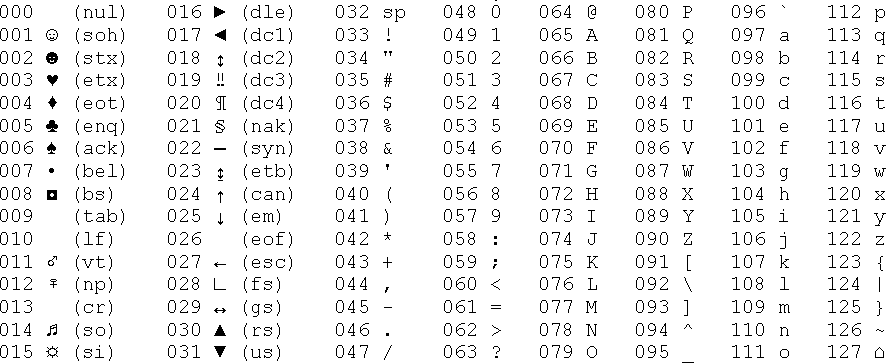
\includegraphics[width=\textwidth]{./img/ascii-table.png} \\ \pause
  
  {\small The table provides an \emph{encoding} scheme from symbols to numbers} \\
  \texttt{72 69 76 76 79} = \texttt{H E L L O} %\pause
  
  %\texttt{'HELLO'}
\end{frame}

%%%%%%%%%%%%%%%%%%%%%%%%%%%%%%%%%%%%%%%%%%%%%%%%%%%%%%%%%%%%%%%%%%%%%%%%%%%%%%%%
\begin{frame}
  \frametitle{How to store text on computer?}
  \Enlarge

  \begin{itemize}
  \myitem \texttt{H E L L O} = \texttt{72 69 76 76 79} \pause
  \myitem  Each symbol is stored individually, one byte long: \\
   \vspace{2mm} \pause
    \begin{tabular}{*{27}{l}}
      72 & \texttt{01001000} \\
      69 & \texttt{01000101} \\
      76 & \texttt{01001100} \\
      76 & \texttt{01001100} \\
      79 & \texttt{01001111} \\
    \end{tabular} \pause
    
    \vspace{2mm}
    {\small \texttt{'HELLO'} : \textcolor{CS101GradBot}{\texttt{01001000 01000101 01001100 01001100 01001111}}}
  \end{itemize}
\end{frame}


%%%%%%%%%%%%%%%%%%%%%%%%%%%%%%%%%%%%%%%%%%%%%%%%%%%%%%%%%%%%%%%%%%%%%%%%%%%%%%%%
\begin{frame}
  \frametitle{Strings}
  \Enlarge

  \begin{itemize} \pause
  \myitem  As a literal:  text surrounded by quotes.
    \begin{itemize}
    \mysubitem  \texttt{'DEEP'}, or \texttt{"DEEP"} \pause
    \mysubitem single quote(\texttt{''}) and double quote (\texttt{""}) are equivalent in python (not in C or C++)
    \end{itemize}\pause
  \myitem  Can have arbitrary length, including an empty string (\texttt{''}). \pause
  \myitem  Each element is a character --- also a string type \pause
  \myitem  In C/C++, a character is a different data type (\texttt{char})
  \end{itemize}
\end{frame}

%%%%%%%%%%%%%%%%%%%%%%%%%%%%%%%%%%%%%%%%%%%%%%%%%%%%%%%%%%%%%%%%%%%%%%%%%%%%%%%%
\begin{frame}
  \frametitle{Strings}
  \Enlarge

  \begin{center}
  \texttt{'the quick brown fox jumps over a lazy dog'}
  \end{center}
 \end{frame}


%%%%%%%%%%%%%%%%%%%%%%%%%%%%%%%%%%%%%%%%%%%%%%%%%%%%%%%%%%%%%%%%%%%%%%%%%%%%%%%%
\begin{frame}
  \frametitle{String operations}
  \Enlarge

  \begin{itemize}
  \myitem  \textbf{Concatenation}:  combine two strings
    \begin{itemize}
    \mysubitem  Uses the \texttt{+} symbol (operator for string concatenation) \pause
    \mysubitem  \texttt{'RACE' + 'CAR'}\pause
    \mysubitem the ``same'' operator works differently with different types of operand (\emph{operator overload})
    \end{itemize}
  \end{itemize} \pause
   \vspace{-1mm}
   \hspace{15mm}\texttt{\textcolor{CS101GradBot}{1 + 2 = 3}} \\ \vspace{1mm}
   \hspace{15mm}\texttt{\textcolor{CS101GradBot}{'RACE' + 'CAR' = 'RACECAR'}} 
\end{frame}


%%%%%%%%%%%%%%%%%%%%%%%%%%%%%%%%%%%%%%%%%%%%%%%%%%%%%%%%%%%%%%%%%%%%%%%%%%%%%%%%
\begin{frame}
  \frametitle{String operations}
  \Enlarge

  \begin{itemize}
  \myitem  \textbf{Repetition}:  repeat a string
    \begin{itemize}
    \mysubitem  Uses the \texttt{*}
    \mysubitem  \texttt{'HELLO '*10}
    \end{itemize}
  \end{itemize}
\end{frame}


%%%%%%%%%%%%%%%%%%%%%%%%%%%%%%%%%%%%%%%%%%%%%%%%%%%%%%%%%%%%%%%%%%%%%%%%%%%%%%%%
\begin{frame}[fragile]
  \frametitle{String operations}
  \Enlarge

  \begin{itemize}
  \myitem  \textbf{Formatting}: Creates string with other data types inserted in \pause
    \begin{itemize}
    %\mysubitem  Formats other data types as a string \pause
    \mysubitem  Requires a special indicator of Formatting: \texttt{\%} \pause
    \mysubitem  Requires indicator of data type
    \end{itemize} \pause
  \begin{semiverbatim}
x = 100 * 54
s = "The value of x is: %\textcolor{CS101GradBot}{i}" % \textcolor{CS101GradBot}{x}
print(s)\pause

\textcolor{CS101GradBot}{The value of x is: 5400}
  \end{semiverbatim}
  \end{itemize}
\end{frame}


%%%%%%%%%%%%%%%%%%%%%%%%%%%%%%%%%%%%%%%%%%%%%%%%%%%%%%%%%%%%%%%%%%%%%%%%%%%%%%%%
\begin{frame}
  \frametitle{Formatting operator}
  \Enlarge

  \begin{itemize}
  \myitem  Creates string with value inserted
    \begin{itemize}
    \mysubitem  Indicators for different data types
      \begin{tabular}{*{27}{ll}}
        \texttt{'\%i'} & \texttt{int} \\
        \texttt{'\%f'} & \texttt{float} \\
        \texttt{'\%e'} & \texttt{float} (scientific notation) \\
        \texttt{'\%s'} & \texttt{str}
      \end{tabular}
    \end{itemize}
  \end{itemize}
\end{frame}

%%%%%%%%%%%%%%%%%%%%%%%%%%%%%%%%%%%%%%%%%%%%%%%%%%%%%%%%%%%%%%%%%%%%%%%%%%%%%%%%
\begin{frame}[fragile]
  \frametitle{Example}
  \Enlarge

  \begin{semiverbatim}
print( 'An integer:  \%i' \% 7 )
print( 'A float:     \%f' \% 7.0 )
print( 'A float:     \%e' \% 7.0 )
print( 'A string:    \%s' \% 'seven' )
  \end{semiverbatim}
\end{frame}

%%%%%%%%%%%%%%%%%%%%%%%%%%%%%%%%%%%%%%%%%%%%%%%%%%%%%%%%%%%%%%%%%%%%%%%%%%%%%%%%
\begin{frame}[fragile]
  \frametitle{Example}
  \Enlarge

  \begin{Verbatim}[commandchars=\\\{\}]
name = "Tao"
grade = 2 / 3
m1 = "Hello, %s!" % name
m2 = "Your grade is:  %f." % grade
print(m1)
print(m2) \pause

\textcolor{CS101GradBot}{
Hello, Tao!}
\textcolor{CS101GradBot}{
Your grade is 0.666667.} 
\end{Verbatim}

\iffalse
\begin{Verbatim}[commandchars=\\\{\}]
m3 = "Your grade is:  %\textcolor{red}{.3}f" % grade
print(m3) \pause

\textcolor{CS101GradBot}{	%CS101PureBase
Your grade is 0.667.}
\end{Verbatim}
\fi

\end{frame} 

%%%%%%%%%%%%%%%%%%%%%%%%%%%%%%%%%%%%%%%%%%%%%%%%%%%%%%%%%%%%%%%%%%%%%%%%%%%%%%%%
\begin{frame}[fragile]
  \frametitle{Example}
  \Enlarge

  \begin{semiverbatim}
x = 3
s = ("%i" % (x+1)) * x**(5%x)
print(s)
  \end{semiverbatim}

  What does this program print?
  \begin{enumerate}[label=\Alph*]
  \item  \texttt{333333333333}
  \item  \texttt{444444444}
  \item  \texttt{9999}
  \item  \texttt{\%i\%i\%i\%i\%i}
  \end{enumerate}
\end{frame}


%%%%%%%%%%%%%%%%%%%%%%%%%%%%%%%%%%%%%%%%%%%%%%%%%%%%%%%%%%%%%%%%%%%%%%%%%%%%%%%%
\begin{frame}
  \frametitle{Escape character \texttt{'\textbackslash'}}
  \Enlarge

  \begin{itemize}
  \myitem Read as "back slash"
  \myitem  Defines special characters
  
    \begin{tabular}{*{27}{l}}
      \texttt{\textbackslash n} & new line \\
      \texttt{\textbackslash t} & tab (tabular key)\\
      \texttt{\textbackslash v} & vertical tab \\
   \end{tabular} \pause
  \myitem De-specialize special characters \pause
  
    \begin{tabular}{*{27}{l}}
      \texttt{\textbackslash \textbackslash} & \texttt{\textbackslash} \\
      \texttt{\textbackslash '} & \texttt{'} \\
      \texttt{\textbackslash "} & \texttt{"} \\
   \end{tabular} 
 \end{itemize} \pause
  
  \hspace{7mm} \textcolor{blue}{\small \texttt{\url{https://docs.python.org/2.0/ref/strings.html}}} 
\end{frame}


%%%%%%%%%%%%%%%%%%%%%%%%%%%%%%%%%%%%%%%%%%%%%%%%%%%%%%%%%%%%%%%%%%%%%%%%%%%%%%%%
\begin{frame}[fragile]
  \frametitle{Example}
  \Enlarge

  \hspace{10mm}Try: \\
  \hspace{12mm}\texttt{\small print('Hello, Tao!\texttt{\textcolor{red}{\textbackslash n}}Your grade is 0.667') \\
  \hspace{12mm}print('3 plus 5 is:\texttt{\textcolor{red}{\textbackslash t}}\%i', \% (3+5)) \\
  \hspace{12mm}print('put .ipynb file in C:\texttt{\textcolor{red}{\textbackslash \textbackslash}}Users\texttt{\textcolor{red}{\textbackslash \textbackslash}}nick')} 
  
  \vspace{3mm}
  \hspace{12mm}\texttt{\small \textcolor{CS101GradBot}{Hello, Tao!\\
  \hspace{12mm}Your grade is 0.667 \\\vspace{1mm}\pause
  \hspace{12mm}3 plus 5 is:\hspace{5mm}8\\\vspace{1mm}\pause
   \hspace{12mm}put .ipynb file in C:\textbackslash Users\textbackslash nick}}
\end{frame}

\iffalse
%%%%%%%%%%%%%%%%%%%%%%%%%%%%%%%%%%%%%%%%%%%%%%%%%%%%%%%%%%%%%%%%%%%%%%%%%%%%%%%%
\begin{frame}
  \frametitle{Quote in Quote}
  \Enlarge

  \begin{itemize}
  \myitem  ``Emily's not coming today'' \pause
  	\begin{itemize}
	\mysubitem \texttt{{\small print('Emily's not coming today')}}
	\mysubitem \texttt{{\small print("Emily's not coming today")}}
	\end{itemize}\pause
  \myitem ``Movie of the week is ''Beauty and Beast''''\pause
  	\begin{itemize}
	\mysubitem \texttt{{\small print('Movie of the week is "Beauty and Beast"')}}
	\mysubitem \texttt{{\small print("Movie of the week is "Beauty and Beast" ")}}
	\end{itemize} \pause
  \myitem rule-of-thumb 
  	\begin{itemize}
	\mysubitem use double quote to enclose single quote
	\mysubitem use single quote to enclose double quote \pause
	\mysubitem use \texttt{\textbackslash '} or \texttt{\textbackslash "} for quotes inside a string
	%\mysubitem sometimes use triple quote (\texttt{''' '''})
	\end{itemize}
 \end{itemize}
\end{frame}
\fi

%%%%%%%%%%%%%%%%%%%%%%%%%%%%%%%%%%%%%%%%%%%%%%%%%%%%%%%%%%%%%%%%%%%%%%%%%%%%%%%%
\begin{frame}[fragile]
  \frametitle{Indexing operator \textbf{[]}}
  \Enlarge

  \begin{itemize}
  \myitem  Extracts single character
\begin{semiverbatim}
a = "FIRE"
a[0]
\end{semiverbatim} \pause
  \myitem  The integer is the index. \pause
  \myitem  \textcolor{red}{We count from zero!} \pause
  \myitem  If negative, counts down from end. \pause
  \myitem \texttt{a[-1]} is the last element
  %\myitem  Does this work on other data types like \texttt{int}?
  \end{itemize}
\end{frame}

%%%%%%%%%%%%%%%%%%%%%%%%%%%%%%%%%%%%%%%%%%%%%%%%%%%%%%%%%%%%%%%%%%%%%%%%%%%%%%%%
\begin{frame}[fragile]
  \frametitle{Question}
  \Enlarge

  \begin{semiverbatim}
s = "ABCDE"
i = (11 % 3) - 7
z = s[i]
  \end{semiverbatim}

  What is the value of \texttt{z}?
  \begin{enumerate}[label=\Alph*]
  \item  \texttt{'A'}
  \item  \texttt{'B'}
  \item  \texttt{'C'}
  \item  \texttt{'D'}
  \item  \texttt{'E'}
  \end{enumerate}
\end{frame}

%%%%%%%%%%%%%%%%%%%%%%%%%%%%%%%%%%%%%%%%%%%%%%%%%%%%%%%%%%%%%%%%%%%%%%%%%%%%%%%%
\begin{frame}[fragile]
  \frametitle{Slicing operator \textbf{:}}
  \Enlarge

  \begin{itemize}
  \myitem  Extracts a range of characters (\emph{substring}) 
  \myitem  Index range specified inside \texttt{[]}
\begin{semiverbatim}
a = "FIREHOUSE"
a[0:4]
\end{semiverbatim} \pause
  \myitem  Can be a bit tricky at first:
    \begin{itemize}
    \mysubitem  Includes character at first index
    \mysubitem  Excludes character at last index
    \end{itemize}
  \end{itemize}
\end{frame}

%%%%%%%%%%%%%%%%%%%%%%%%%%%%%%%%%%%%%%%%%%%%%%%%%%%%%%%%%%%%%%%%%%%%%%%%%%%%%%%%
\begin{frame}[fragile]
  \frametitle{Example}
  \Enlarge

  \begin{semiverbatim}
alpha = "ABCDE"
x = alpha[1:3]
  \end{semiverbatim}
  What is the value of \texttt{x}?
  \begin{enumerate}[label=\Alph*]
  \item  \texttt{'AB'}
  \item  \texttt{'ABC'}
  \item  \texttt{'BC'}
  \item  \texttt{'BCD'}
  \item  \texttt{'CD'}
  \end{enumerate}
\end{frame}

\iffalse
%%%%%%%%%%%%%%%%%%%%%%%%%%%%%%%%%%%%%%%%%%%%%%%%%%%%%%%%%%%%%%%%%%%%%%%%%%%%%%%%
\begin{frame}[fragile]
  \frametitle{Slicing operator \textbf{:} with stepsize}
  \Enlarge

  \begin{itemize}
  \myitem  Extracts a sub-range of characters with a \emph{stepsize}\pause
\begin{semiverbatim}
alpha = "ABCDE"  
alpha[1:3:\textcolor{CS101GradBot}{2}]   \hspace{2mm} \textcolor{CS101GradBot}{\small #last value is stepsize} \pause
'B'
\end{semiverbatim} \pause
\myitem Stepsize can be negative
\begin{semiverbatim}
alpha[4:1:\textcolor{CS101GradBot}{-1}] \pause
'EDC'
\end{semiverbatim}
%alpha[-1:1:\textcolor{CS101GradBot}{-2}]
  \end{itemize}
\end{frame}
\fi


%%%%%%%%%%%%%%%%%%%%%%%%%%%%%%%%%%%%%%%%%%%%%%%%%%%%%%%%%%%%%%%%%%%%%%%%%%%%%%%%
\begin{frame}[fragile]
  \frametitle{Question}
  \Enlarge

  \begin{semiverbatim}
s = "ABCDE"
i = (11 % 3) + 3
z = s[i]
  \end{semiverbatim}

  What is the value of \texttt{z}? \\\vspace{2mm}\pause
  %How about \texttt{s[-5]}?
  \textcolor{red}{\emph{Error}: Out-of-Index!}
\end{frame}


%%%%%%%%%%%%%%%%%%%%%%%%%%%%%%%%%%%%%%%%%%%%%%%%%%%%%%%%%%%%%%%%%%%%%%%%%%%%%%%%
\begin{frame}
  %\frametitle{Complex numbers, $\mathbb{C}$}
  %\Enlarge
  \begin{center}
  \vspace{3mm}
  
\includegraphics[width=1.3\textwidth]{./img/outofindex}\\
  \end{center}
\end{frame}


%%%%%%%%%%%%%%%%%%%%%%%%%%%%%%%%%%%%%%%%%%%%%%%%%%%%%%%%%%%%%%%%%%%%%%%%%%%%%%%%
\section{Functions}

%%%%%%%%%%%%%%%%%%%%%%%%%%%%%%%%%%%%%%%%%%%%%%%%%%%%%%%%%%%%%%%%%%%%%%%%%%%%%%%%
\begin{frame}
  \frametitle{And now for something different...}
  \Enlarge

  \begin{itemize}
  \myitem  A \emph{function} is a piece of code (code block) we can execute with a single line. \pause
    \begin{itemize}
    \mysubitem  Provides an interface that \emph{encapsulates} a series of actions \pause
    \mysubitem  Saves us from rewriting code \pause
    \mysubitem  Makes code cleaner and easy to read \pause
    \mysubitem  Serves as building blocks to build up bigger programs
    \end{itemize} \pause
  \myitem  Analogy:  Functions are like verbs.
  %\myitem  Also called subroutine or procedure.
  \end{itemize}
\end{frame}


%%%%%%%%%%%%%%%%%%%%%%%%%%%%%%%%%%%%%%%%%%%%%%%%%%%%%%%%%%%%%%%%%%%%%%%%%%%%%%%%
\begin{frame}
  \frametitle{Function calls}
  \Enlarge

  \begin{itemize}
  %\myitem  When we want to execute a function, we \emph{call} or \emph{invoke} it. \pause
  \myitem  Use name of the function with parentheses.
    \begin{itemize}
    \mysubitem  \texttt{print()}
    \end{itemize} \pause
  \myitem  Many functions come built-in to Python or in the standard library. \pause
  \myitem  Others we will compose at need.
  \end{itemize}
\end{frame}


%%%%%%%%%%%%%%%%%%%%%%%%%%%%%%%%%%%%%%%%%%%%%%%%%%%%%%%%%%%%%%%%%%%%%%%%%%%%%%%%
\begin{frame}
  \frametitle{Arguments}
  \Enlarge

  \begin{itemize}
  \myitem  Functions can take data as input. \pause
  \myitem  The data that passes to a function is called \emph{Arguments}. \pause
    \begin{itemize}
    \mysubitem  \texttt{print(\textcolor{CS101GradBot}{5})} \pause
    \mysubitem  \texttt{len(\textcolor{CS101GradBot}{'Rex Kwon Do'})} \pause
    \mysubitem  \texttt{abs(\textcolor{CS101GradBot}{-123})} \pause
    \end{itemize}
  \myitem  A function can accept zero to many arguments. \pause
  \myitem  Multiple arguments are separated by commas:
    \begin{itemize}
    %\mysubitem  \texttt{print('10')} \pause
    \mysubitem  \texttt{min(\textcolor{CS101GradBot}{1, 4, 5})}
    \mysubitem  \texttt{max(\textcolor{CS101GradBot}{1, 4, 5})}
    \end{itemize}
  \end{itemize}
\end{frame}

%%%%%%%%%%%%%%%%%%%%%%%%%%%%%%%%%%%%%%%%%%%%%%%%%%%%%%%%%%%%%%%%%%%%%%%%%%%%%%%%
\begin{frame}
  \frametitle{Return value}
  \Enlarge

  \begin{itemize}
  \myitem  Functions can return a result: {\bf return value}. \pause
  \myitem  Return values are the output of a function. \pause
  \begin{itemize}
    \mysubitem  \texttt{a = min(1, 4, 5)}
    \mysubitem  \texttt{b = max(1, 4, 5)} \pause
  \end{itemize}
  \myitem Can return nothing 
  \begin{itemize}
    \mysubitem  \texttt{print(5)} \pause
    \mysubitem  \texttt{a = print(5)} \pause
    \mysubitem a is a \texttt{'\textcolor{CS101GradBot}{NoneType}'}
  \end{itemize} 
  \end{itemize}
\end{frame}

%%%%%%%%%%%%%%%%%%%%%%%%%%%%%%%%%%%%%%%%%%%%%%%%%%%%%%%%%%%%%%%%%%%%%%%%%%%%%%%%
\begin{frame}[fragile]
  \frametitle{Example}
  \Enlarge

 
  \begin{semiverbatim} 
\textcolor{red}{def} f(x)\textcolor{red}{:}
    y = x**2 
    area = 0.5*math.pi * y 
    return area
  \end{semiverbatim}

\end{frame}

%%%%%%%%%%%%%%%%%%%%%%%%%%%%%%%%%%%%%%%%%%%%%%%%%%%%%%%%%%%%%%%%%%%%%%%%%%%%%%%%
\begin{frame}[fragile]
  \frametitle{Example}
  \Enlarge

 
  \begin{semiverbatim} 
def \textcolor{red}{f}(x):
    y = x**2 
    area = 0.5*math.pi * y
    return area
  \end{semiverbatim}

\end{frame}

%%%%%%%%%%%%%%%%%%%%%%%%%%%%%%%%%%%%%%%%%%%%%%%%%%%%%%%%%%%%%%%%%%%%%%%%%%%%%%%%
\begin{frame}[fragile]
  \frametitle{Example}
  \Enlarge

 
  \begin{semiverbatim} 
def f(\textcolor{red}{x}):
    y = x**2 
    area = 0.5*math.pi * y
    return area
  \end{semiverbatim}

\end{frame}

%%%%%%%%%%%%%%%%%%%%%%%%%%%%%%%%%%%%%%%%%%%%%%%%%%%%%%%%%%%%%%%%%%%%%%%%%%%%%%%%
\begin{frame}[fragile]
  \frametitle{Example}
  \Enlarge

 
  \begin{semiverbatim} 
def f(x):
    \textcolor{red}{y = x**2} 
    \textcolor{red}{area = 0.5*math.pi * y} 
    return area
  \end{semiverbatim}

\end{frame}

%%%%%%%%%%%%%%%%%%%%%%%%%%%%%%%%%%%%%%%%%%%%%%%%%%%%%%%%%%%%%%%%%%%%%%%%%%%%%%%%
\begin{frame}[fragile]
  \frametitle{Example}
  \Enlarge

 
  \begin{semiverbatim} 
def f(x):
    y = x**2
    area = 0.5*math.pi * y
    \textcolor{red}{return} \textcolor{CS101PureBase}{area}
  \end{semiverbatim}

\end{frame}

%%%%%%%%%%%%%%%%%%%%%%%%%%%%%%%%%%%%%%%%%%%%%%%%%%%%%%%%%%%%%%%%%%%%%%%%%%%%%%%%
\begin{frame}
  \frametitle{Type conversion}
  \Enlarge

  \begin{itemize}
  \myitem  A set of built-in functions to convert data from one type to another. \pause
    \begin{itemize}
    \mysubitem  \texttt{float('3.14')} 
    %\mysubitem  \texttt{float('3.00e-2')} \pause
    \mysubitem  \texttt{str(3.14)}
    \mysubitem  \texttt{int(3.14)} 
    \end{itemize} \pause
  \myitem  Be careful of nonsense:
    \begin{itemize}
    \mysubitem  \texttt{int('Rex')}
    \mysubitem  \texttt{int(3 + 5j)}
    \end{itemize}
  \end{itemize}
\end{frame}

%%%%%%%%%%%%%%%%%%%%%%%%%%%%%%%%%%%%%%%%%%%%%%%%%%%%%%%%%%%%%%%%%%%%%%%%%%%%%%%%
\begin{frame}
  \frametitle{User input}
  \Enlarge

  \begin{itemize}
  \myitem  \texttt{x = input()} \pause
  \myitem  Takes keyboard input typed by user \pause
  \myitem  Return value:  keyboard input from user (as \texttt{str})
  \myitem  No argument to the function \pause
  \begin{itemize}
  	\mysubitem \textcolor{CS101GradBot}{cannot skip the parentheses! }
  \end{itemize}
  \end{itemize}
\end{frame}


\iffalse
%%%%%%%%%%%%%%%%%%%%%%%%%%%%%%%%%%%%%%%%%%%%%%%%%%%%%%%%%%%%%%%%%%%%%%%%%%%%%%%%
\begin{frame}
  \frametitle{Goal}
  \Enlarge

  \begin{itemize}
  %\myitem  A program should achieve a goal.
  \myitem  Next time we will start writing our own python program.
  \end{itemize}
\end{frame}
\fi


%%%%%%%%%%%%%%%%%%%%%%%%%%%%%%%%%%%%%%%%%%%%%%%%%%%%%%%%%%%%%%%%%%%%%%%%%%%%%%%%
\section{Reminders}

%%%%%%%%%%%%%%%%%%%%%%%%%%%%%%%%%%%%%%%%%%%%%%%%%%%%%%%%%%%%%%%%%%%%%%%%%%%%%%%%
\begin{frame}
  \frametitle{Reminders}
  \Enlarge

  \begin{itemize}
  \myitem Homework \#2 is due Tuesday Oct.\ 3. \pause
  \myitem Opps, no class next week
  \end{itemize}
\end{frame}

\end{document}
